\documentclass{article}
\usepackage{verbatim}
\usepackage[scale=0.75,top=2cm]{geometry}
\usepackage{tabularx}
\usepackage{algpseudocode}
\usepackage{multicol}
\usepackage{caption}
\usepackage{tikz}
\usepackage[utf8]{inputenc}
\usepackage{longtable}
\usepackage{array}
\usepackage{floatrow}
\usepackage{blindtext}
\usepackage{caption}
\usepackage{graphicx}
\usepackage{booktabs}
\newfloatcommand{capbtabbox}{table}[][\FBwidth]
\usetikzlibrary{shapes}



\begin{document}
%----------------------------------------------------------------------------------------------------------------------------------------
\title{Project Report}
\author{Akshat Bisht 40053762}
\date{\today}
\maketitle
%----------------------------------------------------------------------------------------------------------------------------------------

\newpage
%----------------------------------------------------------------------------------------------------------------------------------------


\section{Introduction}
Graph coloring is defined as, assignment of "colors" to certain objects in a graph subject to certain constraints.
There are different types of graph coloring,such as, Vertex coloring, Edge Coloring, Face coloring (planar).
 In this paper, we deal with on-line Vertex coloring, which is defined as 
coloring vertices of a graph such that no two adjacent vertices share the same color.\\

$^{[1]}$An on-line coloring is a coloring algorithm that immediately colors the vertices of a graph G taken from a list without looking ahead or changing colors already assigned. To be precise, an on-line coloring algorithm of G is an algorithm that properly colors G by recieving its vertices in some order $v_1,v_2,v_3...v_n$. The color of $v_i$ assigned by looking at the subgraph of G induced by the set $\{v_1,v_2...v_i\}$, and the color of $v_i$ never changes during the algorithm.\\

Some common applications of Graph Coloring include Job Scheduling, Register Allocation and Sudoku Solving.\\

In this paper, we narrow our focus on the problem of Bipartite Graphs coloring.
We compare the performance of 3 graph coloring algorithms. 
Two of them are well known (i.e First Fit and CBIP), the third algorithm (MyAlgorithm) is similar to CBIP but uses randomization when
 assigning color. We run these algorithms and compare their performance with graphs of different sizes. Some graphs were created by the author itself using the Erdős–Rényi model, while the other were taken from the Network Repository.\\

 We observe that First Fit, eventhough is known to theoretically to perform worse that CBIP, performs is very comparable to CBIP in our testing.
First Fit also seems to give us a very stable set results in all the graphs that we tested.
CBIP is seen to give us a very erratic results when it comes to the Network Repository graphs. 
 The randomized version of CBIP, introduced by us, does seem to give us a little bit of improvement over the original CBIP.


\section{Background} 

$^{[2]}$Coloring  theory  started  with  the  problem  of  coloring  the countries of a map in such a way that no two countries that have a common border receive the same color.  If we denote the countries by points in the plane and connect each pair of points that correspond to countries with a common border by a curve, we obtain a planar graph. The celebrated Four Color Problem  asks  if  every  planar  graph  can  be  colored  with  4 colors.  It seems to have been mentioned for the first time inwriting in an 1852 letter from A. De Morgan to W.R. Hamilton. Nobody thought at that time that it was the beginning of a new theory. The first ”proof” was given by Kempe in 1879. It stood for more than 10 years until Heawood in 1890 found a mistake.   Heawood proved that five colors are enough to color any map.  The Four Color Problem became one of the most difficult problems in Graph Theory. Besides colorings it stimulated many other areas of graph theory. Generally, coloring theory is the theory about conflicts:  adjacent vertices in a graph always must have distinct colors, i.e.  they are in a permanent conflict. If we have a ”good” coloring, then we respect all the conflicts. If we have a ”bad” coloring, then we have a pair of adjacent vertices colored with the same color. This  looks  like  having  a  geographic  map  where  some  two countries having common border are colored with the samecolor. Graphs  are  used  to  depict  ”what  is  in  conflict  with what”, and colors are used to denote the state of a vertex. So, more precisely, coloring theory is the theory of ”partitioning the sets having internal unreconcilable conflicts” because we will only count ”good” colorings.

\newpage

\section{New Algorithm}

This is where you describe your algorithm that you propose that is different from FirstFit and CBIP. You will evaluate this 
algorithm alongside FirstFit and CBIP.
\bigbreak
The Algorithm that we have implemented for this project isn't a greedy based algorithm, thus it is different from FirstFit. The algorithm's
computation procedure is similar to the CBIP algorithm except that at the end it uses \textbf{randomization}.\\
The Psuedocode for the is Algorithm is presented below.
		
	\begin{multicols}{2}% 2-column layout
	  \begin{minipage}{0.45\textwidth}
	    \begin{algorithmic}[1]% Taken from the algorithmicx package documentation
	      \Procedure{MyAlgorithm}{$G,\sigma$}
	      \State Initialize Set \textit{$S_c$}.
	      \State Compute $C_v \mbox{ - connected component of } v$
	      \State Compute bipartition of $C_v = S_v \cup \widetilde{S_v}$
	      \State \ \ \ \  v $\in S_v$ and $N(v) \subseteq \widetilde{S_v}$
	      \State $S_c$= colors \textbf{not} in $\widetilde{S_v} \mbox{ but present in } S_v$
	      \State Color \textit{i} = Randomly selected out of $S_c$.
	      \State Color v with \textit{i}
	      \EndProcedure
	    \end{algorithmic}
	  \end{minipage}
	The Breadth First Search Algorithm is used to separate all the vertices that are in the $S_v$ and $\widetilde{S_v}$ . 
	The Set $S_c$ contains set of all the vertices/colors that are not in $\widetilde {S_v}$ but are in $S_v$ is created.
	 A color is selected randomly from $S_c$  and assigned to the vertex.\\

	 In CBIP, we select color with the minimum color value from the set. But in our algorithm, the color is selected randomly from the set.

	\end{multicols}	


\section{Implementation Details}

\bigbreak
The implementation details of the code can be broken down into the following sections.\\

\textbf{Graph Representation:}\\

The graphs that can be successfully read by the program, should be in the same format as mentioned in the project.pdf (i.e MMC format). 
The code uses and adjacency matrix of boolean type to read the graphs that are inputted. The cells in the matrix are set to true if an edge exists
between the nodes. The use of an adjacency matrix helps making sure that the graphs that are being read are automatically converted to Bipartite 
Graphs(i.e \textit{Duplicating method}). A disadvantage of this method is that a lot of memory is wasted and this method may not be optimal for larger graphs or for machines with low memory.\\


\textbf{Important Methods and Variables :}\\

\textit{ReadNetworkRepoGraphs() }: Reads all the graphs downloaded from the Network Repository website.The extension of the files are
 "NetworkRepoGraph1.txt", "NetworkRepoGraph2.txt"... You can change the number of graphs to read to check the result by running the inner
 loop once instead of 5 times. If it is changed to 1 , then it will read only "NetworkRepoGraph1.txt" and you can check the results of 1 graph with 
the lowest number of nodes more carefully. \\ 

 \textit{ReadRandomGraphs() }: Reads all the graphs downloaded from the Random Graphs created by the class "RandomGraphs.java".The
 extension of the files are"RandomGraph1.txt", "RandomGraph2.txt"... You can change the number of graphs to read to check the result by 
running the inner loop once instead of 5 times. If it is changed to 1 , then it will read only "NetworkRepoGraph1.txt" and you can check the
 results of 1 graph with the lowest number of nodes more carefully.\\

\textit{createGraph()}:In the class "RandomGraphs.java", the createGraph() method, has an array with different integer values (number of nodes).
 An adjacency matrix is created and as we iterate through the 2D-boolean array. Initailly all values are False(no edge exist between nodes)
 by default. There is an in-built Java random function that produces integer values in the interval [1,11]. While being on a cell if the randomizer spits out an even number, the cell value is turned True (edge exists). Thus, $P(edge)= \frac{2}{5}$ and $P(\widetilde{edge})=\frac{3}{5}$.\\ 

\textit{RandomOrderInput()}: It fills up an array with all integer values in the interval [1,numberOfVertices], and then all the values in the array are
randomly shuffled using the Java randomizer.\\

\textit{Data()}: Prints the average of the number of colors used by each algorithm for each graph by using respectively. A graphical representation 
of this data is shown in the Result section of this report.\\

\textit{Iterations}: This global variable can be changed, depending upon how many times the user want to run all 3 algorithms for all the inputted 
graphs and see what the averaged out values of the number of colors used by all algorithms for all the graphs will be. We ran 100 iterations and the 
average values computed are in a table in the result section of this report.\\

\textbf{Challenges :}\\

The most challenging part of this project was the coding of CBIP algorithm. The algorithm took some time to understand properly, but thanks to the
 Professor Pankratov and his Teaching Assistant(Ali Mohammed) we were able to grasp the concept. Coding the Breadth-First-Search(BFS)  
and keeping alternating depth level vertices in different sets was the most challenging, algorithmically speaking. \\

Some other challenges we faced in this program were due to extensive use of arrays in our program, we had to be really careful as most of the errors
 came from ArrayIndexOutOfBoundsException because array indices start from 0 while the vertices in the graphs start from 1.\\

Initially the code was tested with small graphs containing 5 to 10 nodes, as computing solutions of these graphs by hand was feasible to compare
 with the answers computed by the code. These small graphs were created to try and get the most number of colors from the FirstFit and CBIP algorithms (Adversarial Input). These graphs are also submitted with code.\\ 

We cannot be completely sure that this program is bug free. The input graph formats and graph naming conventions have to be correct, for the 
code to function as intended. We may have missed some edge cases. But because of extensive testing we are confident that the
 algorithmic executions are correct. 

\section{Experimental Details}

\textit{\textbf{System Specification : }}
This program was coded in Java programming language using Java version 14.
The system was coded and tested in Windows operating system,with 16 Gigabytes of RAM and with an i5 processor.
The code was written in the Eclipse IDE. \\
\newpage
\textit{\textbf{Input Graphs Details: }}

\begin{center}
 \begin{tabular}{||p{3cm} | p{4cm} | p{2cm}|p{2cm} ||} 
\hline
\multicolumn{4}{|c|}{Network Repository Graphs} \\

 \hline

 Graph Name& File Name & Nodes & Edges \\ [0.5ex] 
 \hline\hline
 dwt\_66$^{[3]}$ &NetworkRepoGraph1.txt & 66 &193  \\ 
 \hline
 GD06\_theory$^{[4]}$&NetworkRepoGraph2.txt  & 101 & 190\\
 \hline
can\_144$^{[5]}$ &NetworkRepoGraph3.txt  & 144 & 720 \\
 \hline
 cat\_ears\_3\_1$^{[6]}$&NetworkRepoGraph4.txt & 204 & 542\\
 \hline
  ash219$^{[7]}$&NetworkRepoGraph5.txt  & 219 &438\\ [1ex] 
 \hline
\end{tabular}
\end{center}

\begin{center}
 \begin{tabular}{||p{3cm} | p{4cm} | p{2cm}|p{2cm} ||} 
\hline
\multicolumn{4}{|c|}{Random Graphs} \\

 \hline

 Graph Name& File Name & Nodes & Edges \\ [0.5ex] 
 \hline\hline
 RandomGraph1 &RandomGraph1.txt & 25 & 137  \\ 
 \hline
 RandomGraph2 & RandomGraph2.txt  & 50 & 603 \\
 \hline
RandomGraph3 & RandomGraph3.txt  & 100 & 2,307 \\
 \hline
 RandomGraph4 & RandomGraph4.txt & 200 & 8,989\\
 \hline
RandomGraph5 & RandomGraph5.txt  & 400 & 36,317\\ [1ex] 
 \hline
\end{tabular}
\end{center}

%------------------------------------------------------------------------


\begin{comment}

		\begin{center}
		 \begin{tabular}{||p{2.5cm} | p{0.8cm} | p{1.5cm} | p{1.5cm} | p{1.9cm} ||} 
		\hline
		\multicolumn{5}{|c|}{Network Repository Graphs} \\
		 \hline
		\hline
		Graph Name& Nodes & \multicolumn{3}{|c|}{Colors} \\
		\hline
		 & & FirstFit & CBIP & MyAlgorithm \\ [0.5ex] 
		 \hline\hline
		 & 66 & 4.91 & 17.5 & 17.53 \\ 
		 \hline
		 & 101 & 6.41 & 3.08 & 3.08 \\
		 \hline
		 & 144 & 9.41 & 32.49 & 32.49 \\
		 \hline
		 & 204 & 6.36 & 29.05 & 28.23 \\
		 \hline
		 & 219 & 6.23 & 22.81 & 23.61\\ [1ex] 
		 \hline
		\end{tabular}
		\end{center}
		
		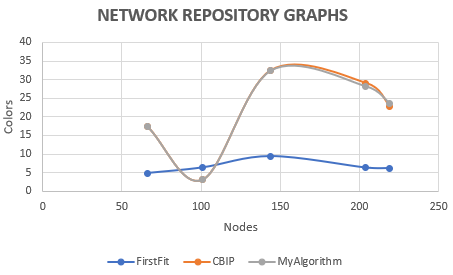
\includegraphics[width=0.75\textwidth]{NetworkRepoGraph}
		
		
		\begin{center}
		 \begin{tabular}{||p{2cm} | p{2cm} | p{2cm} | p{2cm} ||} 
		\hline
		\multicolumn{4}{|c|}{Random Graphs} \\
		\hline
		\hline
		 Nodes & \multicolumn{3}{|c|}{Colors} \\
		\hline
		 & FirstFit & CBIP & MyAlgorithm \\ [0.5ex] 
		 \hline\hline
		 25 & 7.89 & 8.03 & 7.99 \\ 
		 \hline
		 50 & 14.02 & 14 & 13.58\\
		 \hline
		 100 & 21.94 & 21.93 & 21.04 \\
		 \hline
		 200 & 36.25 & 36.41 & 34.59 \\
		 \hline
		 400 & 62.88 & 63.19 & 60.16\\ [1ex] 
		 \hline
		\end{tabular}
		\end{center}
		
		\bigbreak
		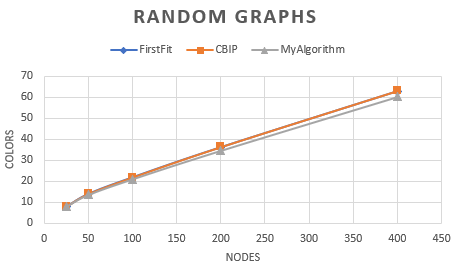
\includegraphics[width=0.75\textwidth]{RandomGraph}

\end{comment}

%------------------------------------------------------------------------

\section{Results}

\bigbreak
This section of the report is divided into 2 sections : Network Graph Data and Random Graph Data. \\

\textbf{\textit{Random Graph Data:}}
Selected Random Graphs and their details are mentions in the previous section of this report. The following table and graph represent the data 
that was collected. These results were generated after 100 iterations on same graphs but using different random input order.
%------------------------------------------------------------------------

	\begin{minipage}{0.5\linewidth}
		 \begin{tabular}{||p{2.5cm} | p{0.8cm} | p{1.5cm} | p{1.5cm} | p{1.9cm} ||} 
			\hline
			\multicolumn{5}{|c|}{Random Graphs} \\
			\hline
			\hline
			Graph Name& Nodes & \multicolumn{3}{|c|}{Colors} \\
			\hline
			 & & FirstFit & CBIP & MyAlgorithm \\ [0.5ex] 
			 \hline\hline
			RandomGraph1 & 25 & 7.89 & 8.03 & 7.99 \\ 
			 \hline
			RandomGraph2 & 50 & 14.02 & 14 & 13.58\\
			 \hline
			RandomGraph3 & 100 & 21.94 & 21.93 & 21.04 \\
			 \hline
			RandomGraph4 & 200 & 36.25 & 36.41 & 34.59 \\
			 \hline
			RandomGraph5 & 400 & 62.88 & 63.19 & 60.16\\ [1ex] 
			 \hline
		\end{tabular}
	\end{minipage}\hfill
	\begin{minipage}{5cm}
		\centering
		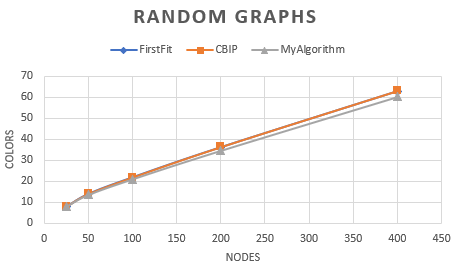
\includegraphics[height=5cm,width=7cm]{RandomGraph}
	\end{minipage}
\bigbreak
We can observe from the following data that, all three algorithms have a very similar performance. MyAlgorithm has perfomed a little better than
FirstFit and CBIP, so can see that use of Randomness has helped. We can observe that the introduction of Randomness benifitted us. 
The CBIP and FirstFit have almost similar results. \\

\bigbreak

\textbf{\textit{Network Graph Data:}}
Selected Network Graphs and their details are mentions in the previous section of this report. The following table and graph represent the data 
that was collected. Similarto the Random Graphs, the results were generated after 100 iterations on same graphs but using different random 
input order.\\

\bigbreak
	\begin{minipage}{0.5\linewidth}
		 \begin{tabular}{||p{2.5cm} | p{0.8cm} | p{1.5cm} | p{1.5cm} | p{1.9cm} ||} 
			\hline
			\multicolumn{5}{|c|}{Network Repository Graphs} \\
			 \hline
			\hline
			Graph Name& Nodes & \multicolumn{3}{|c|}{Colors} \\
			\hline
 		 	& & FirstFit & CBIP & MyAlgorithm \\ [0.5ex] 
 			\hline\hline
			 dwt\_66$^{[3]}$& 66 & 4.91 & 17.5 & 17.53 \\ 
			 \hline
 			 GD06\_theory$^{[4]}$& 101 & 6.41 & 3.08 & 3.08 \\
 			\hline
			can\_144$^{[5]}$ & 144 & 9.41 & 32.49 & 32.49 \\
			 \hline
			 cat\_ears\_3\_1$^{[6]}$& 204 & 6.36 & 29.05 & 28.23 \\
 			\hline
 			ash219$^{[7]}$& 219 & 6.23 & 22.81 & 23.61\\ [1ex] 
 			\hline
		\end{tabular}
	\end{minipage}\hfill
	\begin{minipage}{5cm}
		\centering
		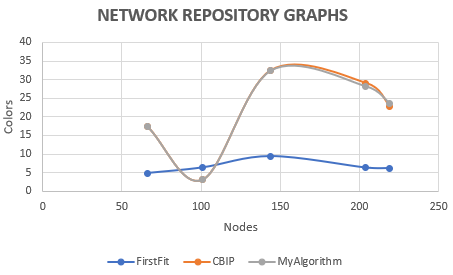
\includegraphics[height=5cm,width=7cm]{NetworkRepoGraph}
	\end{minipage}

%------------------------------------------------------------------------

We can observe from the following data that, FirstFit usually performs better and is more stable than CBIP and MyAlgorithm. The CBIP and 
MyAlgorithm performance is very similar. We can observe that the introduction of Randomness hasn't benifitted us. The greedy based approach
works well for the Network Repository Graphs. \\


We also observe that 2 major factors affect the performance of these algorithms i.e  Input Order and Graph Density.
\bigbreak
\textit{Input Order} : We can easily show that with use of an adversarial input, CBIP will perform better than FirstFit, but since we use a Random 
input order, it seems to work towards the advantage of FirstFit.\\
\bigbreak
\textit{Graph Density} : Intuitively, the denser the graph(more edges between nodes), the worst FirstFit should perform. While CBIP
should perform better than FirstFit, but due to a Random Input Order in our experiment FirstFit does better if not the same.\\ 

MyAlgorithm seems to perform better, if not the same as CBIP. This shows that Randomness does help, if not in all cases. 



\section{Future Directions}


In the future we would like to use additional graph parameters such as average degree of vertices in our experimental set up. We can extend these coloring techniques to planar  graph coloring problems(eg. 3D Coloring) as well. We also would like to continue and see
 where else we can use randomness in color selection. Initially, we wanted to implement a randomized online graph coloring algorithm proposed 
by Sundar Vishwanathan in "Randomized online graph coloring"$^{[6]}$, but due inability to get the paper we couldn't produce it.\\

One of the major limitations for this project is that we used a very limited sample space.We could have used larger graphs(with more number of
vertices), and  the creation of Random Graphs in our project had produced very dense graphs probably because the probablility was set at 0.4 
to an edge to be added. This caused very dense graphs to be created, we would like to test our code with sparse graphs by reducing the probability. 
\newpage

\section{Bibliography}

\begin{enumerate}
	
	\item On-Line and First Fit Coloring of Graphs, A.Gyárfás and J.Lehel, Computer and Automation Institute, Hungarian Academy Of Sciences. 
	
	\item Graph Coloring: History, results and open problems,Vitaly I. Voloshin, 2009, Troy University, Troy, AL

	\item dwt-66,SYMMETRIC CONNECTION TABLE FROM DTNSRDC, WASHINGTON, G. Everstine, D. Taylor, Miscellaneous Networks,
			 The Network Data Repository with Interactive Graph Analytics and Visualization, Ryan A. Rossi and Nesreen K. Ahmed

	\item GD-06\_Theory,Graph Drawing Contest, Pajek network,2006, Miscellaneous Networks,
			 The Network Data Repository with Interactive Graph Analytics and Visualization, Ryan A. Rossi and Nesreen K. Ahmed

	\item can-144,SYMMETRIC PATTERN FROM CANNES,LUCIEN MARRO,JUNE 1981,
 			The Network Data Repository with Interactive Graph Analytics and Visualization,Ryan A. Rossi and Nesreen K. Ahmed

	\item cat-ears-3-1, Combinatorial optimization as polynomial eqns, Susan Margulies, UC Davis ,2008, Miscellaneous Networks,
			 The Network Data Repository with Interactive Graph Analytics and Visualization, Ryan A. Rossi and Nesreen K. Ahmed

	\item ash219,UNSYMMETRIC OVERDETERMINED PATTERN OF HOLLAND SURVEY. ASHKENAZI,1974 ,Miscellaneous Networks,
			 The Network Data Repository with Interactive Graph Analytics and Visualization, Ryan A. Rossi and Nesreen K. Ahmed


  	\item Randomized Online Graph Coloring, Sundar Viswanathan, Mathematics, Computer Science, J.Algorithms, 1992.
\end{enumerate}




\newpage



\end{document}